%//------ Section 03 -------------------------------------------------------------------------------------------------
\chapter{Complementary materials for the analysis:\\Analysis of the correlated production of strange hadrons}
\label{appendix:CorrelatedAnalysis}
%//-----------------------------------------------------------------------//

\section{Comparison between measurements and models}

The model comparison articulates around two pictures, two approaches to describe the small and large systems: \Pythia and \Epos. The former relies its description of the hadronisation processes on the Lund string model, while the other employs a core-corona model. In the next paragraphs, each of these models will be introduced in details, and most particularly the hadronisation mechanisms used in the model comparison to the results.

\subsection{\Pythia}

\Pythia's hadronisation mechanisms are based solely on the Lund string model. The starting point of this framework is the spring-like nature of the QCD interaction between two quarks, supported by lattice QCD studies (\Sec\ref{subsubsec:confinement}, and in particular \eq\ref{eq:QCDPotential}). 

The gluon field between two colour charges can be viewed as a colour flux tube, a string of tension $\kappa \simeq 1$ \gev/\fm with a potential energy increasing linearly with the distance between the quarks \cite{bierlichComprehensiveGuidePhysics2022}. As the partons move apart, their kinetic energy is progressively converted into potential energy, until it has been fully transferred to the string . At this point, the string reaches its maximal extension, $E/2\kappa$, and the partons move back to their starting point and meet again. The string has completed a full period. This so-called \say{yo-yo} motion corresponds to a meson in the Lund string picture. If the partons move further apart than the maximum, the original string breaks up giving rise to a new $q \bar{q}$ pair\footnote{The typical break-up time of a string is about 2 \fmC \cite{bierlichComprehensiveGuidePhysics2022}.}. It is through this mechanism that mesons are produced. In order to form a baryon, the string must fragment into diquark--anti-diquark pairs\footnote{Any quark flavour can be obtained in principle, but the heavier the quark, the more suppressed it is. For instance, the production of light flavour quarks is almost inexpensive, while strange and charm quarks have to pay a suppression factor of $0.3$ and $10^{-11}$. Consequently, the yield of heavy quark flavour can basically be ignored with the string breaking mechanism, they are produced in other processes in the perturbative regime of QCD \cite{sjostrandIntroductionPYTHIA2015}.}. 

This picture received further developments over the years, amongst the most important: the multiparton interaction (MPI) model and the colour reconnection (CR) mechanisms. The former stems from the composite nature of the hadrons, that leads possibly to several parton-parton interactions when colliding two hadrons \cite{sjostrandDevelopmentMPIModelling2017}. The MPI model basically comprises all the processes involving multiple partons. The CR mechanisms allow colour strings in \textit{causal contact}\footnote{This point is extremely important as the space-time separation between two MPIs is not taken into account by default.} to re-arrange and form a different configuration. An example of colour reconnection is the string junction, which opens the way towards additional mechanisms for baryon production as illustrated in \fig\ref{fig:BaryonProductionMechanisms} \cite{heleniusRecentPythiaDevelopments2016}.\\

\begin{figure}[t]
%\centering
\hspace*{-1.25cm}
\subfigure[]{
	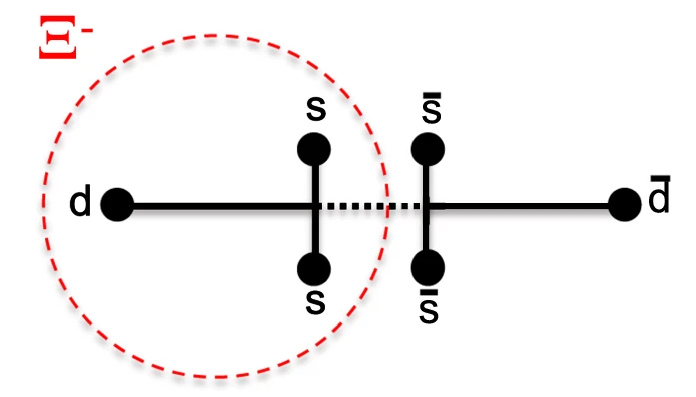
\includegraphics[width=0.55\textwidth, valign=t]{Figs/Chapter6/BaryonFormation_StringBreaking.png}
	\label{fig:StringBreaking}
} 
\subfigure[]{
	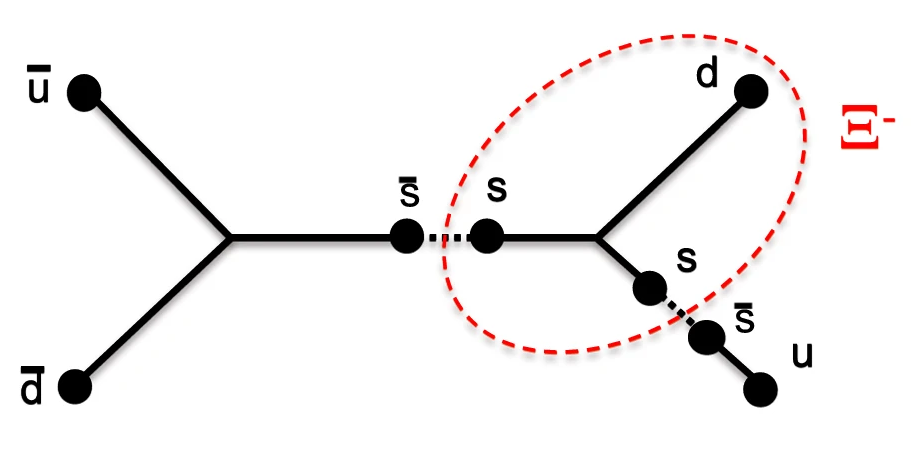
\includegraphics[width=0.6\textwidth, valign=t]{Figs/Chapter6/BaryonFormation_StringJunction.png}
	\label{fig:StringJunction}
} 
\caption{Baryon production mechanism within the \Pythia framework, in the case of a \rmXiM hyperon: (a) the colour string fragments into a diquark--anti-diquark pairs; (b) two strings form a junction, that breaks down into a $s\bar{s}$ pair. Figure taken from \cite{adolfssonQCDChallengesPp2020}.}
	\label{fig:BaryonProductionMechanisms}
\end{figure}

\Pythia has historically focused on electroweak and hard QCD processes, parton shower, hadronisation, particularly in small systems where no QGP formation is considered. The discovery of long-range particle correlations in high-multiplicity pp collisions in 2010 \cite{cmscollaborationObservationLongRangeNearSide2010}\cite{chatrchyanObservationLongrangeNearside2013}\cite{rolandLongrangeCorrelationsHigh2015}, followed by the observation of the strangeness enhancement in small systems in 2017 \cite{alicecollaborationEnhancedProductionMultistrange2017}, forced to re-consider the QGP-like effects in pp collisions. The aforementioned models could offer a qualitative description of some of those effects, while being completely off on some other observables like the anisotropic flow. New developments were needed. To that end, additional interactions between the strings have \say{recently} been implemented, namely the rope hadronisation (or also refered as colour rope) and string shoving \cite{bierlichComprehensiveGuidePhysics2022}.

The rope hadronisation follows somehow the same idea as the string junction, namely that strings may form in a cluster of partons. When multiple strings overlap, their colour fields act coherently, forming a stronger field. These cluster of strings can then be viewed as a string with an effective tension $\tilde{\kappa}$ greater than $\kappa$, that is a colour rope. This increased string tension leads to an increase\footnote{This increase actually depends on the colour configuration of the different strings. Quarks with the same colour charges can form a coherent state, increasing $\tilde{\kappa}$; whereas, with opposite/incoherent colour charges, they combine into an anti-colour, thus reducing $\tilde{\kappa}$.} of the strangeness production (or equivalently, it decreases its suppression factor), that can subsequently be used to model the strangeness enhancement.

Another effect of the overlapping of strings is the string shoving. Strings occupying the same volume can interact together. It turns out that they dominantly repel each other, resulting in a shoving pressure. Each hadron later receives its share of the push, which leads ultimately to a flow of hadrons, mimicing the anisotropic flow effects.

\subsection{\Epos}

Originally designed to reproduce heavy-ion interactions, \Epos employs a core-corona model, a unique approach when all the other high-energy physics MC generators (\Pythia, \Herwig, etc) are corona-like models. 

The basic idea behind this framework starts with the observation that a hadron-hadron collision corresponds in fact to many elementary collisions happening simultaneously, that can be modelled via the formation of parton ladders -- similar to the MPI concept, describing the multiple parton scatterings -- or (cut-)Pomerons\footnote{A Pomeron -- named after Isaak Pomeranchuk -- is a concept incorporated by Vladimir Gribov into the Regge theory, developed by Tullio Regge in 1959 \cite{reggeIntroductionComplexOrbital1959}. This theory attempts to describe the total cross section of hadronic collisions at high energies, at a time when the quark model does not exist yet. In this theory, a particle and all its excitations -- for instance, the \rhoMes meson spin-1, spin-3, spin-5, etc -- lie on the same trajectory, the Regge trajectory. Each resonance contributes to the scattering amplitudes; their combined contribution is viewed as an exchange of an object named Reggeon \cite{levinEverythingReggeonsPart1998}. Although the Regge theory provides a good description of the total cross section at low energies, it predicts a decreasing trend at high energies while it is in fact flat. The solution to this problem is brought by Gribov, who introduces a new Reggeon: the Pomeron. In modern particle physics, the Pomeron corresponds to various processes at high energy, such as a parton ladder. \Epos' main theoretical tool being the S-matrix theory inspired by the Gribov-Regge picture \cite{wernerCorecoronaProcedureMicrocanonical2023}, it is not surprising to encounter the concept of parton ladder in such phenomenological model. One can distinguish two sorts of Pomeron: the cut and the uncut version. Basically, the latter corresponds to an elastic contribution to the scattering amplitude, whereas the former represents an inelastic contribution \cite{wernerMonteCarloEvent2022}.}. It turns out the parton ladder can be viewed as a colour flux tube, a string like in the Lund string model that breaks via the production of a $q\bar{q}$ pair into string segments often referred as \say{pre-hadrons}. These serves as initial conditions for the hadronisation.

\begin{figure}[t]
\centering
	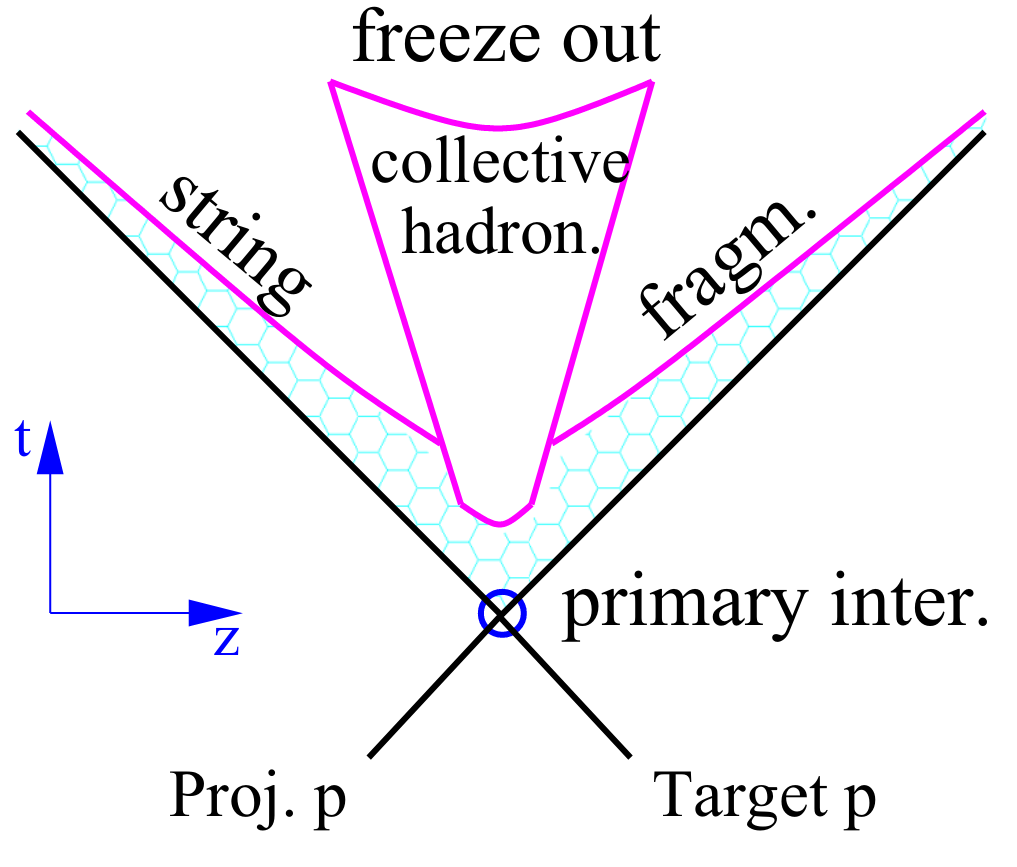
\includegraphics[width=0.55\textwidth, valign=t]{Figs/Chapter6/medium.png}
\caption{Schematic representation of the space-time evolution of the particle production in a hadron-hadron collision. The central cone represents the core part where the hadrons undergo a collective hadronisation at the freeze-out surface. The hyperbola line encompasses the corona surrounding the core; the string segments in this region  hadronise via string fragmentation. Figure taken from \cite{pierogEPOSLHCTest2015}.}
	\label{fig:CoreCorona}
\end{figure}

Based on these pre-hadrons, the core-corona procedure illustrated in \fig\ref{fig:CoreCorona} comes into play. In the regions with a high density (above a certain threshold, easily reached in heavy-ion collisions) of string segments, these may overlap and fuse into a fluid. This corresponds to the \say{core} of the system as opposed to the \say{corona}, usually located in the peripheral regions of the system (by definition), where the string density is lower. The pre-hadrons in the core loose their energy and evolve according to hydrodynamics, until the energy density falls below a critical value. At this stage, the fluid undergoes a collective hadronisation via a micro-canonical procedure\footnote{The string segments constituting the core are gathered in different clusters for each pseudo-rapidity bin. The hadronisation is performed in each cluster separately using the micro-canonical ensemble formalism \cite{pierogEPOSLHCTest2015}.} at the freeze-out surface (\fig\ref{fig:CoreCorona}), in order to ensure energy, momentum and flavour conservations. The formed hadrons receive a Lorentz boost according to the radial and longitudinal expansions of the fluid core. For what concerns the string segments in the corona part, they hadronise through string fragmentations as in \Pythia.\\

This presentation of \Epos corresponds to the current implementation of the model, \EposFour. This procedure is applied for simulating both pp and heavy-ion collisions. Thereby, this model assumes the formation of, at least, a QGP droplet in small systems (\fig\ref{fig:CoreCoronaPbPbpp}). There exists also different configurations that considers only the \say{core} or the \say{corona}.

\begin{figure}[t]
\centering
\subfigure[]{
	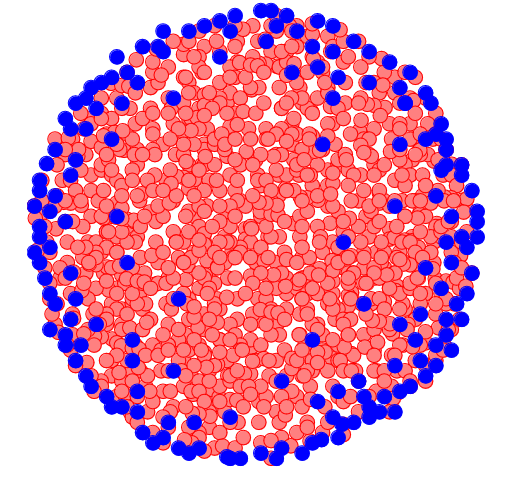
\includegraphics[width=0.35\textwidth, valign=t]{Figs/Chapter6/CoreCoronaPbPb.png}
}
\subfigure[]{
	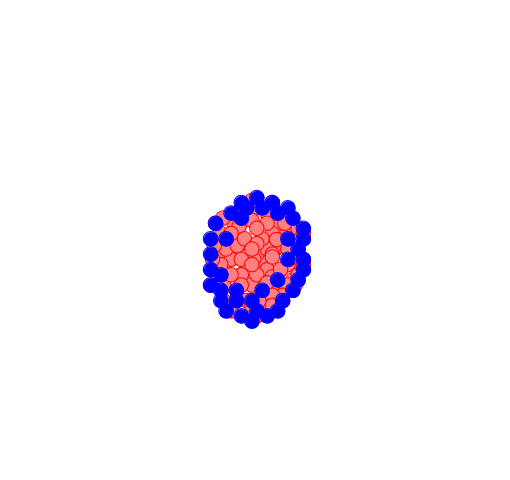
\includegraphics[width=0.35\textwidth, valign=t]{Figs/Chapter6/CoreCoronapp.png}
}
\caption{Schematic representation of the pre-hadrons distributions in a large system such as a Pb-Pb collision (a) and in a small system like a pp collision (b). The red dots represents the pre-hadrons in the core, while the blue ones belong to the corona. Figures taken from \cite{wernerCorecoronaProcedureMicrocanonical2023}.}
	\label{fig:CoreCoronaPbPbpp}
\end{figure}

\section{\Epos configuration}
\begin{verbatim}
!-------------------------------------------------------------
!  proton-proton parameterized fluid expansion (mimic hydro)
!    much faster than full hydro
!-------------------------------------------------------------

application hadron !hadron-hadron, hadron-nucleus, or nucleus-nucleus
set laproj 1       !projectile atomic number
set maproj 1       !projectile mass number
set latarg 1       !target atomic number
set matarg 1       !target mass number
set ecms 13000     !sqrt(s)_pp

set istmax 25
set iranphi 1
ftime on

set ihepmc 1
!set nfull 10           !number of events


!suppressed decays:
nodecays
 110 20 2130 -2130 2230 -2230 1130 -1130 1330 -1330 2330 -2330 3331 -3331
end

set ninicon 1            !number of initial conditions used for hydro evolution
core PFE                 !parameterized fluid expansion (mimic hydro) : PFE, full, off
hydro off                !hydro not activated (hlle, off)
eos off                  !eos not activated (x3ff, off)
hacas full               !hadronic cascade activated  (full, off)

set nfreeze 1            !number of freeze out events per hydro event
set modsho 1             !certain printout every modsho events
set centrality 0         ! 0=min bias

!print * 2                !printout of event to ...check file

!-----put here online analysis part----
!       see expl1,2,3
!--------------------------------------
\end{verbatim}

\section{\Pythiaeight, Monash 2013 configuration}

\begin{verbatim}
#Beams
Beams:idA = 2212 ! Proton
Beams:idB = 2212

# Min. bias
#SoftQCD:all = on

# Min. bias alternative
SoftQCD:nonDiffractive = on
SoftQCD:singleDiffractive = on
SoftQCD:doubleDiffractive = on

# random seed
Random:setSeed = on
Random:seed = 0

# Set cuts
# Use this for hard leading-jets in a certain pT window
PhaseSpace:pTHatMin = 0   # min pT
PhaseSpace:pTHatMax = 13000   # max pT

# Use this for hard leading-jets in a certain mHat window
PhaseSpace:mHatMin = 0   # min mHat
PhaseSpace:mHatMax = $SQRTS   # max mHat

# Makes particles with c*tau0 > 10 mm stable: (default value = 10.0 in mm / Here = 10 m)
# See http://home.thep.lu.se/~torbjorn/pythia81html/ParticleDecays.html
# tau0 = seems to deal with particle species by species, i.e. selection based on 'cTau(PDG)'
ParticleDecays:limitTau0 = On
ParticleDecays:tau0Max = 10000.0

# Set tune
Tune:pp=14
\end{verbatim}

\section{\Pythiaeight, configuration with colour reconnection enabled}
\begin{verbatim}
# Parameter of the MPI model to keep total multiplicity reasonable
MultiPartonInteractions:pT0Ref = 2.15

# Parameters related to Junction formation/QCD based CR
BeamRemnants:remnantMode = 1
BeamRemnants:saturation = 5
ColourReconnection:mode = 1
ColourReconnection:allowDoubleJunRem = off
ColourReconnection:m0 = 0.3
ColourReconnection:allowJunctions = on
ColourReconnection:junctionCorrection = 1.2
ColourReconnection:timeDilationMode = 2
ColourReconnection:timeDilationPar = 0.18

# Enable rope hadronization
Ropewalk:RopeHadronization = on

# Also enable string shoving, but don't actually do anything.
# This is just to allow strings to free stream until hadronization
# where the overlaps between strings are calculated.
Ropewalk:doShoving = on
Ropewalk:tInit = 1.5 # Propagation time
Ropewalk:deltat = 0.05
Ropewalk:tShove = 0.1
Ropewalk:gAmplitude = 0. # Set shoving strength to 0 explicitly

# Do the ropes.
Ropewalk:doFlavour = on

# Parameters of the rope model
Ropewalk:r0 = 0.5 # in units of fm
Ropewalk:m0 = 0.2 # in units of GeV
Ropewalk:beta = 0.1

# Enabling setting of vertex information is necessary
# to calculate string overlaps.
PartonVertex:setVertex = on
PartonVertex:protonRadius = 0.7
PartonVertex:emissionWidth = 0.1
\end{verbatim}


